\documentclass{standalone}
\usepackage{graphicx}
\usepackage{pgf,tikz}
\usepackage{pgfplots}
\usepackage[europeanresistors,americaninductors]{circuitikz}
\usetikzlibrary{spy}
\begin{document}


\begin{tikzpicture}

\def\buff at (#1,#2){
	
	\draw[very thick](-5+#1, -0.5+#2) rectangle (7+#1,6.5+#2);
	\node[anchor=center] at (5+#1, 3.7+#2) {Displayscreen};
	\draw(3.5+#1,1.5+#2) rectangle (6.5+#1,3.5+#2);
	
	\node[anchor=center] at (0.5+#1, 5.2+#2) {Buffer1};
	\draw(-1+#1,3+#2) rectangle (2+#1,5+#2);
	
	\node[anchor=center] at (0.5+#1, 2.2+#2) {Buffer2};
	\draw(-1+#1,0+#2) rectangle (2+#1,2+#2);
	
	\node[anchor=center] at (0.5+#1, 5.9+#2) {Memory};
	\draw(-1.2+#1,-0.2+#2) rectangle (2.2+#1,5.7+#2);
	
	\node[anchor=center] at (-4+#1, 2.5+#2) {Processor};
}



% first write
\node[anchor=center] at (0.5, 4) {Hello World};
\draw[->,>=stealth](-3,2.5)--(-1.2,4) node[midway,above, sloped] {\footnotesize write data};
\draw[->,>=stealth](2.2,1)->(3.5,2.5) node[midway,above, sloped] {\footnotesize show buffer};


% second write
\node[anchor=center] at (14+0.5, 4) {Hello World};
\node[anchor=center] at (14+5, 2.5) {Hello World};
\draw[->,>=stealth](14+-3,2.5)--(14+-1.2,1) node[midway,above, sloped] {\footnotesize write data};
\draw[->,>=stealth](14+2.2,4)->(14+3.5,2.5) node[midway,above, sloped] {\footnotesize show buffer};
\draw[->,>=stealth, gray, dashed](-3+14,2.5)--(-1.2+14,4);
\draw[->,>=stealth, gray, dashed](2.2+14,1)->(3.5+14,2.5);
\draw[->,>=stealth, gray, dashed](-1.5+14,3.5)arc(10:-15:4);
\draw[->,>=stealth, gray, dashed](2.5+14,1.75)arc(15:-12:-4);

\node[inner sep=0pt] at (14.5,1)
{
\includegraphics[width=3cm, height=2cm]{iceage.jpg}};




% third write
\draw[->,>=stealth](-3,2.5-9)--(-1.2,4-9) node[midway,above, sloped] {\footnotesize write data};
\draw[->,>=stealth](2.2,1-9)->(3.5,2.5-9) node[midway,above, sloped] {\footnotesize show buffer};
\draw[->,>=stealth, gray, dashed](-3,2.5-9)--(-1.2,1-9);
\draw[->,>=stealth, gray, dashed](2.2,4-9)->(3.5,2.5-9);

\node[inner sep=0pt] at (0.5,1-9)
{
\includegraphics[width=3cm, height=2cm]{iceage.jpg}};
\node[inner sep=0pt] at (5,2.5-9)
{
\includegraphics[width=3cm, height=2cm]{iceage.jpg}};
\node[inner sep=0pt] at (0.5,4-9)
{
\includegraphics[width=3cm, height=2cm]{iceage.jpg}};

\draw[<-,>=stealth, gray, dashed](-1.5,3.5-9)arc(10:-15:4);
\draw[<-,>=stealth, gray, dashed](2.5,1.75-9)arc(15:-12:-4);
\node[anchor=center,red] at (0.75, 4.5-9) {\textbf{New Text}};



% fourth write
\draw[->,>=stealth](-3+14,2.5-9)--(-1.2+14,1-9) node[midway,above, sloped] {\footnotesize write data};
\draw[->,>=stealth](2.2+14,4-9)->(3.5+14,2.5-9) node[midway,above, sloped] {\footnotesize show buffer};
\draw[->,>=stealth, gray, dashed](-3+14,2.5-9)--(-1.2+14,4-9);
\draw[->,>=stealth, gray, dashed](2.2+14,1-9)->(3.5+14,2.5-9);

\draw[->,>=stealth, gray, dashed](-1.5+14,3.5-9)arc(10:-15:4);
\draw[->,>=stealth, gray, dashed](2.5+14,1.75-9)arc(15:-12:-4);

\node[inner sep=0pt] at (0.5+14,4-9)
{
\includegraphics[width=3cm, height=2cm]{iceage.jpg}};
\node[inner sep=0pt] at (5+14,2.5-9)
{
\includegraphics[width=3cm, height=2cm]{iceage.jpg}};
\node[inner sep=0pt] at (0.5+14,1-9)
{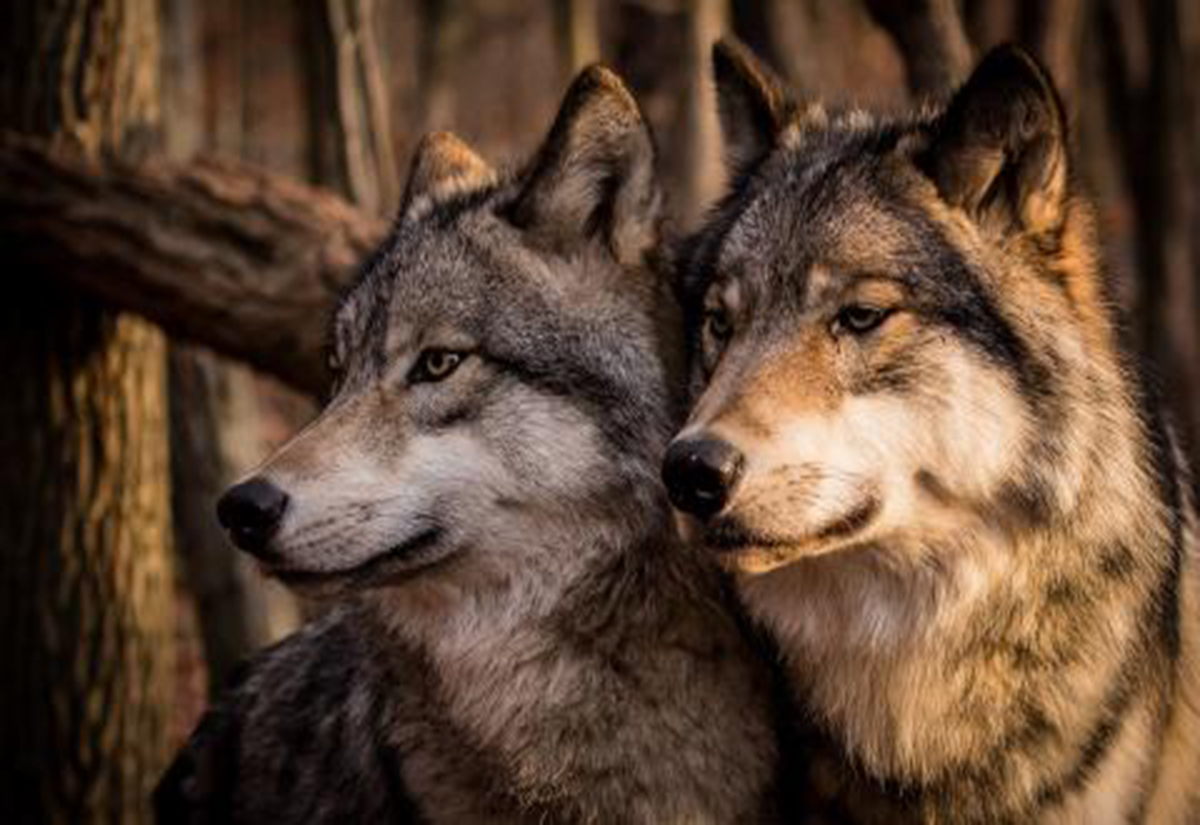
\includegraphics[width=3cm, height=2cm]{02.jpg}};

\node[anchor=center,red] at (0.75+14, 4.5-9) {\textbf{New Text}};
\node[anchor=center,red] at (0.25+14+5, 4.5-9-1.5) {\textbf{New Text}};

  \begin{scope}
%\draw [step=0.03,very thin] (-1, 5.9) grid (-0.79, 6.26);

\buff at (0,0);
\buff at (14,0);
\buff at (0,-9);
\buff at (14,-9);
\draw[->,>=stealth,very thick](7,2.5)--(9,2.5);
\draw[->,>=stealth,very thick](9,-0.5)--(7,-2.5);
\draw[->,>=stealth,very thick](7,2.5-9)--(9,2.5-9);

\node[] at (0.5, -0.8) {Step 1: Write data in buffer1};
\node at (14.5, -0.8) {Step 2: Write data in buffer2 and show buffer1 on display};

\node[] at (0.5, -2.2) {Step 3: Write data in buffer1 and show buffer 2 on display};
\node at (14.5, -2.2) {Step 4: Write data in buffer2 and show buffer1 on display};
\end{scope}


\end{tikzpicture}
\end{document}
